% !TEX root = ../discriminative_filtering.tex

\section{Preface}
This chapter is primarily my work, but was definitely inspired by the survey of~\textcite{Che13}.  Books have been written on this topic alone, e.g. \textcite{Wie49,Jaz70,And79,Str90,Sar13}, with applications including the Apollo program~\cite{Hal66, Bat70, Gre10}, aircraft guidance~\cite{Sch70}, GPS navigation~\cite{Hof01}, weather forecasting~\cite{Bue17}, and---of course---neural filtering (covered later), so I tried here to provide a digestible, salient overview.  

\section{Introduction}
Consider a state space model for $Z_{1:T}:=Z_1,\dotsc,Z_T$ (latent states) and $X_{1:T}:=X_1,\dotsc,X_T$ (observations) represented as a Bayesian network:
\[
\begin{CD}
Z_1 @>>> \cdots @>>>  Z_{t-1} @>>> Z_t @>>> \cdots  @>>> Z_T \\
@VVV @.	@VVV @VVV @. @VVV \\
X_1  @. @. X_{t-1} @. X_t @. @. X_T
\end{CD}
\]
The conditional density of $Z_t$ given $X_{1:t}$ can be expressed recursively using the Chapman--Kolmogorov equation and Bayes' rule \cite{Che03}
\begin{equation} \label{e:s1:BF}
p(z_t|x_{1:t}) \propto p(x_t|z_t) \int p(z_t|z_{t-1})\; p(z_{t-1}|x_{1:t-1}) \; dz_{t-1}
\end{equation}
where the proportionality constant involves an integral over $z_t$.  To be more explicit, we can re-write~\eqref{e:s1:BF} as follows:
\begin{subequations} \label{e:s1:BFalt}
\begin{gather} p(z_t|x_{1:t-1}) = \textstyle \int p(z_t|z_{t-1}) p(z_{t-1}|x_{1:t-1}) \; dz_{t-1} , \label{e:s1:BFa} \\
p(z_t|x_{1:t}) = \frac{p(x_t|z_t)p(z_t|x_{1:t-1})}{\int p(x_t|z_t) p(z_t|x_{1:t-1}) \; dz_t}. \label{e:s1:BFb}
\end{gather}  
\end{subequations}

\subsection{Methodology Taxonomy}

Modeling these conditional probabilities and solving or approximating the integrals in \eqref{e:s1:BFalt} constitutes Bayesian filtering.  We taxonomize filtering methods according to how the integral in \eqref{e:s1:BF} is computed.  This mirrors closely the ways that Bayesians perform inference in general.  To filter, one may:

\begin{enumerate}
    \item \emph{Use a model with an exact solution}, such as the Kalman filter~\cite{Kal60,Kal61}, or the model specifications of \textcite{Ben81} or \textcite{Dau84,Dau86}.  These models entail no approximation and integration is done in closed form.
    
    \item \emph{Employ a variational method that replaces the current model with a closely-related tractable one}.  For example, the extended Kalman filter and the statistically-linearized filter fit a generic model to a linear model that then integrates exactly~\cite{Gel74,Sar13}.  One can also approximate an arbitrary distribution as the sum of Gaussians and then handle each Gaussian component analytically~\cite{Als72}.  Alternatively, integration can be done via a Laplace transform~\cite{Koy10}.  These similar methods have many names in the literature, including the Gaussian assumed density filter,
    Series expansion-based filters, Fourier--Hermite Kalman filter~\cite{Sar12}.  The model is approximated, but then integration can be done exactly.
    
    \item \emph{Integrate using a quadrature rule}.  In this category we include sigma-point filters such as the Unscented Kalman Filter~\cite{Jul97,Wan00,van04} and also Quadrature Kalman filters~\cite{Ito00,Ito00b} and  Cubature Kalman filters~\cite{Ara07,Ara09}.  Under these models, integrals are approximated based on function evaluations at deterministic points.
    
    \item \emph{Integrate with Monte Carlo}.  Such approaches are called Sequential Monte Carlo or particle filtering~\cite{Ham54,Gor93}.  These methods apply to all classes of models, but tend to be the most expensive and suffer the curse of dimensionality~\cite{Dau03}.  Integration is done with a Monte Carlo approximation; the models do not need to be approximated.
    
\end{enumerate}

%%%%%%%%%%%%%%%%%%%%%%%%%%%%%%%%%%%%%%%%%%%%%%%%%
\section{Exact Filtering with the Kalman Filter (KF)} \index{Kalman Filter}

The Kalman filter specifies a linear, Gaussian relationship between states and observations to yield an analytic solution that can be efficiently computed.  Here we derive the classic Kalman updates~\cite{Kal60,Kal61}.

\subsection{Model} \label{s:KF:mdl}
Let $\eta_d(z;\mu,\Sigma)$ denote the $d$-dimensional multivariate Gaussian distribution with mean vector $\mu\in\RR^{d\times 1}$ and covariance matrix $\Sigma\in\SS_d$ evaluated at $z\in\RR^{d\times 1}$, where $\SS_d$ denotes the set of $d\!\times\!d$ positive definite (symmetric) matrices.
Assume that the latent states are a stationary, Gaussian, vector autoregressive model of order one; namely, for $A\in\RR^{d\times d}$ and $S,\Gamma\in\SS_d$,   
\begin{subequations} \label{e:s1:KFstateproc}
\begin{align}
 p(z_0) & = \eta_d(z_0;0,S), \label{e:s1:KFstationary} \\ 
 p(z_t|z_{t-1}) & = \eta_d(z_t;Az_{t-1},\Gamma), \label{e:s1:KFpred} 
\end{align}
\end{subequations}
For observations in ${\cal{X}}=\RR^{n\times 1}$ and for fixed $H\in\RR^{n\times d}$, $b\in\RR^{n\times 1}$, and $\Lambda\in\SS_n$, we have
\begin{equation} \label{e:s1:KFobs}
p(x_t|z_t) = \eta_n(x_t;Hz_t+b,\Lambda).
\end{equation}

\subsection{Inference}
Under the above model, we see that the posterior at each step will be Gaussian so we may adopt the ansatz:
\begin{equation} \label{e:s1:KFposterior}
p(z_t|x_{1:t}) = \eta_d(z_t; \nu_t, \Phi_t).
\end{equation}
We solve for $\nu_t$ and $\Phi_t$ recursively using~\eqref{e:s1:BF}:
\begin{align} 
p(z_t|x_{1:t}) 
&\propto \eta_n(x_t;Hz_t+b,\Lambda) \int \eta_d(z_t;Az_{t-1},\Gamma) \eta_d(z_{t-1}; \nu_{t-1}, \Phi_{t-1}) \; dz_{t-1} \\
&\propto \eta_n(x_t;Hz_t+b,\Lambda)\; \eta_d(z_t;A\nu_{t-1},A\Phi_{t-1}A^\intercal + \Gamma) \label{e:s1:BF_Kalman}.
\end{align}

Setting
\begin{align}
\hat \nu_{t-1} &= A\nu_{t-1} \label{e:s1:hat_nu},\\
\hat \Phi_{t-1} &= A\Phi_{t-1}A^\intercal + \Gamma, \label{e:s1:hat_phi}
\end{align}
we have
\begin{align} 
p(z_t|x_{1:t}) 
&\propto \eta_n(x_t;Hz_t+b,\Lambda)\; \eta_d(z_t;\hat\nu_{t-1},\hat\Phi_{t-1}) \label{e:s1:KF_deriv_start}\\
&\propto e^{-(x_t-Hz_t-b)^\intercal\Lambda^{-1}(x_t-Hz_t-b)/2} e^{-(z_t-\hat\nu_{t-1})^\intercal\hat\Phi_{t-1}^{-1}(z_t-\hat\nu_{t-1})/2} \\
&\propto e^{-z_t^\intercal H^\intercal \Lambda^{-1}Hz_t/2+z_t^\intercal H ^\intercal \Lambda^{-1}(x_t-b)-z_t^\intercal\hat\Phi_{t-1}^{-1} z_t/2 +z_t^\intercal \hat\Phi_{t-1}^{-1}\hat\nu_{t-1}} \\
&\propto e^{-z_t^\intercal (H^\intercal \Lambda^{-1}H + \hat\Phi_{t-1}^{-1})z_t/2+z_t^\intercal (H ^\intercal \Lambda^{-1}(x_t-b)+\hat\Phi_{t-1}^{-1}\hat\nu_{t-1})} \\
&\eta_d\big(z_t; \Phi_t(H ^\intercal \Lambda^{-1}(x_t-b)+\hat\Phi_{t-1}^{-1}\hat\nu_{t-1}), \Phi_t \big)
\end{align}
where
\begin{align}
\Phi_t 
&= (H^\intercal \Lambda^{-1}H + \hat\Phi_{t-1}^{-1})^{-1} \\
&= \hat\Phi_{t-1} - \hat\Phi_{t-1}H^\intercal(H\hat\Phi_{t-1}H^\intercal + \Lambda)^{-1}H\hat\Phi_{t-1} \\
&= (I_d - \hat\Phi_{t-1}H^\intercal(H\hat\Phi_{t-1}H^\intercal + \Lambda)^{-1}H)\hat\Phi_{t-1} \label{e:s1:phit_reln}
\end{align}
due to the Woodbury matrix identity, where $I_d$ is the $d$-dimensional identity matrix.  Many textbook derivations define the Kalman gain
\begin{equation} \label{e:s1:Kalman_gain}
K_t := \hat\Phi_{t-1}H^\intercal(H\hat\Phi_{t-1}H^\intercal + \Lambda)^{-1}
\end{equation}
so that
\begin{equation} \label{e:s1:Kalman_var}
\Phi_t 
= (I_d - K_tH)\hat\Phi_{t-1}
\end{equation}
and
\begin{equation} \label{e:s1:Kalman_mean}
\nu_t = \hat\nu_{t-1} + K_t(x_t -b - H\hat\nu_{t-1}).
\end{equation}
These are the traditional Kalman updates~\cite{Kal60}.  Kalman's original paper does not assume Gaussian dynamics; however under the Gaussian modeling assumptions, this filter yields exact solutions to~\eqref{e:s1:BF}.

\subsection{Remark}
Note that the Kalman model implies
\begin{equation}
p(z_t|x_{1:t-1}) = \eta_d(z_t;\hat\nu_{t-1},\hat\Phi_{t-1})
\end{equation}
so that
\begin{equation}
p(x_t|x_{1:t-1})= \eta_n(x_t;H\hat\nu_{t-1}+b,H\hat\Phi_{t-1}H^\intercal+\Lambda).
\end{equation}
Let $\bar X_t, \bar Z_t$ be distributed as $X_t,Z_t$ conditioned on $X_{1:t-1}$, respectively.  Then
\begin{align}
\var[\bar X_t] &= H\hat\Phi_{t-1}H^\intercal+\Lambda, \\
\operatorname{Cov}[\bar Z_t, \bar X_t] &= \hat\Phi_{t-1}H^\intercal,
\end{align}
so we can re-write~\eqref{e:s1:Kalman_gain},~\eqref{e:s1:Kalman_var}, and~\eqref{e:s1:Kalman_mean} as
\begin{align}
K_t &= \operatorname{Cov}[\bar Z_t, \bar X_t] (\var[\bar X_t])^{-1} \label{e:s1:KF_gain_alt}, \\
\Phi_t 
& = \var[\bar Z_t] - K_t \var[\bar X_t] K_t^\intercal \label{e:s1:KF_var_alt}, \\
\nu_t &= \mathbb{E}[\bar Z_t] + K_t(x_t - \mathbb{E}[\bar X_t]). \label{e:s1:KF_mean_alt}
\end{align}
This will form the basis for the Gaussian assumed density filter.

\subsection{Related Work}
\textcite{Ben81} and \textcite{Dau84,Dau86,Dau05} extended the families of models under which \eqref{e:s1:BF} may be solved exactly.  In the case that the state space is finite, the grid-based method also provides an exact solution~\cite{Seg76,Mar79,Ell94,Ell94b,Aru02,Kal16}.  The underlying idea is that when there are only a finite number of states, a particle filter with a particle for each state makes \eqref{e:s1:PF} an exact representation for the posterior density, and such a representation can be updated exactly~\cite{Aru02}.

%%%%%%%%%%%%%%%%%%%%%%%%%%%%%%%%%%%%%%%%%%%%%%%%%
\begin{figure}[h]
\begin{minipage}[t]{.45\textwidth}
\includegraphics[width=\linewidth]{apollo_landing}
\caption[A photo from the Apollo 11 Lunar Landing]{The Apollo Lunar Module used a variant of the Kalman Filter to land Neil Armstrong on the moon~\cite{Hal66,Hoa69,Bat70}.  Image credit: \textsc{NASA}.}
\end{minipage}%
\hfill
\begin{minipage}[t]{.45\textwidth}
\includegraphics[width=\linewidth]{earth_rise}
\caption[Earthrise]{GPS receivers use the Extended Kalman filter to model and mitigate satellite clock offset and atmospheric delays~\cite{Axe95,Hof01}. Image credit: \textsc{NASA}.}
\end{minipage}
\end{figure}

%%%%%%%%%%%%%%%%%%%%%%%%%%%%%%%%%%%%%%%%%%%%%%%%%
\section{Model Approximation with the Extended Kalman Filter} \label{s:EKF} \index{Extended Kalman Filter}

This approach expands the model from Section~\ref{s:KF:mdl} and performs inference by finding the closest tractable model and using it instead. \index{integration techniques!variational}

\subsection{Model} \label{s:EKF:mdl}
We extend our model now to allow the relationship between the latent states and observations to be nonlinear:  
\begin{equation} \label{e:s1:EKFobs}
p(x_t|z_t) = \eta_n(x_t;h(z_t),\Lambda)
\end{equation}
where $h:\RR^d \to \RR^n$ is a differentiable function. We use the same state process as in Section~\ref{s:KF:mdl}, namely
\begin{subequations}
\begin{align}
 p(z_0) & = \eta_d(z_0;0,S), \\ 
 p(z_t|z_{t-1}) & = \eta_d(z_t;Az_{t-1},\Gamma).
\end{align}
\end{subequations}
Many of the original derivations and references include a nonlinear, Gaussian state update the state model as well.  The way that inference is adapted to allow for nonlinearity is identical for both the measurement and state models, so we discuss only the measurement model here.

\subsection{Inference}
We may approximate the solution to \eqref{e:s1:BF} in the same form as \eqref{e:s1:KFposterior}
by linearizing the function $h:\RR^d\to\RR^n$ around $\hat \nu_{t-1}$ (from Equation~\ref{e:s1:hat_nu}):
\begin{equation} \label{e:s1:EKF_h_approx}
h(z_t) \approx h(\hat \nu_{t-1}) + \tilde H (z_t - \hat \nu_{t-1})
\end{equation}
where $\tilde H \in\RR^{n\times d}$ is given component-wise for $1\leq i \leq n$ and $1 \leq j \leq d$ as
\begin{equation}
\tilde H_{ij} = \tfrac{\partial}{\partial z_j} h_i(z) \big\vert_{z=\hat \nu_{t-1}}.
\end{equation}
With this Taylor series approximation, we then take
\begin{align}
p(x_t|z_t) 
&= \eta_n(x_t; h(\hat \nu_{t-1}) + \tilde H (z_t - \hat \nu_{t-1}), \Lambda) \\
&= \eta_n(x_t ; \tilde H z_t + h(\hat \nu_{t-1}) -\tilde H \hat \nu_{t-1}, \Lambda) \\
&= \eta_n(\tilde x_t; \tilde H z_t + \tilde b, \Lambda)
\end{align}
where $\tilde b =  h(\hat \nu_{t-1}) -\tilde H \hat \nu_{t-1}$.  This problem is now identical to that of the original Kalman filter, where $H,b$ have been replaced by $\tilde H, \tilde b$, respectively.  Thus, the updated equations (Equations~\ref{e:s1:Kalman_gain},~\ref{e:s1:Kalman_var}, and~\ref{e:s1:Kalman_mean} for the KF) become
\begin{align}
K_t &= \hat\Phi_{t-1}\tilde H^\intercal(\tilde H\hat\Phi_{t-1}\tilde H^\intercal + \Lambda)^{-1} \label{e:s1:ekf_gain}, \\
\Phi_t &= (I_d - K_t\tilde H)\hat\Phi_{t-1} \label{e:s1:ekf_phi}, \\
\nu_t &= \hat\nu_{t-1} + K_t(x_t - h(\hat\nu_{t-1}) ) \label{e:s1:ekf_nu}.
\end{align}

\subsection{Related Work}
Instead of a first order Taylor series approximation, it is also possible to use statistical linearization within the EKF framework~\cite{Gel74,Sar13}.  The resulting filter is aptly named the statistically linearized filter.  With $Z\sim\N(0,S)$, parameters for the linear approximation are chosen to minimize the MSE
\begin{equation}
\hat b, \hat A := \argmin_{b,A}\{\Exp[(h(Z)-(\hat b + \hat A Z))^\intercal (h(Z)-(\hat b + \hat A Z))]\}
\end{equation}
yielding
\begin{align}
\hat b & = \Exp[h(Z)]\\
\hat A & = \Exp[h(Z) Z^\intercal] S^{-1}
\end{align}
The approximation 
\begin{equation}
h(x)\approx \hat b + \hat A x
\end{equation}
is then used in place of~\eqref{e:s1:EKF_h_approx}.


It is also possible to use a second-order expansion~\cite{Ath68, Gus12}.  Alternatively, one can use a Fourier-Hermite series representation in the EKF framework~\cite{Sar12}.

\subsection{The Iterative EKF (IEKF)} \index{Extended Kalman Filter!Iterative}
This approach iteratively updates the center point of the Taylor series expansion used in the EKF to obtain a better linearization \cite{Fri66,Wis69}.  In place of \eqref{e:s1:ekf_gain}, \eqref{e:s1:ekf_phi}, and \eqref{e:s1:ekf_nu}, the IEKF updates are initialized by $\nu_t^0=\hat\nu_{t-1}$ and $\Phi_t^0=\hat\Phi_{t-1}$ and then proceed as follows:
\begin{align}
H^{i+1} &= h'(\nu_t^i) \label{e:s1:iekf_slope} \\
K_t^{i+1} &= \hat\Phi_{t-1} (H^{i+1})^\intercal( H^{i+1} \hat\Phi_{t-1} (H^{i+1})^\intercal + \Lambda)^{-1} \label{e:s1:iekf_gain}, \\
\Phi_t^{i+1} &= (I_d - K_t^{i+1}H^{i+1})\hat\Phi_{t-1} \label{e:s1:iekf_phi}, \\
\nu_t^{i+1} &= \hat\nu_{t-1} + K_t^{i+1}(x_t - h(\nu_t^i) -H^{i+1}(\hat\nu_{t-1}-\nu_t^i)) \label{e:s1:iekf_nu}.
\end{align}
\textcite{Bel93} showed that this algorithm is equivalent to iterative Gauss--Newton updates to place $\nu_t$ at the MAP for $Z_t$.  Finding the MAP can be done with other iterative methods as well, e.g. Levenberg--Marquardt or progressive correction~\cite{Fat12}.  Iterative techniques have been applied to other filters~\cite{Mur14}.  The iterative EKF itself was extended to the Backward-Smoothing Kalman Filter~\cite{Psi05,Psi13}.

%%%%%%%%%%%%%%%%%%%%%%%%%%%%%%%%%%%%%%%%%%%%%%%%%
\section{Model Approximation with Laplace-based Methods} \index{integration techniques!Laplace approximation}

The Laplace approximation performs integration by replacing an integrand $f$ with a Gaussian centered at the maximum of $f$ matching the curvature of $f$ at that point~\cite{Kas90,But07}.  Such a method can be used generally for for Bayesian inference~\cite{Koy10,Qua15}.

\subsection{Laplace Approximation} \label{s:Laplace}
The Laplace approximation can be used to approximate the integrals in Equation~\ref{e:s1:BF}.  At step $t$,
\begin{align*}
p(z_t | x_{1:t})  
& \propto p(x_t | z_t) \int p(z_t|z_{t-1})\ p(z_{t-1} | x_{1:t-1})\ dz_{t-1} \\
& = p(x_t | z_t)\ p(z_t| x_{1:t-1}) =: r(z_t)
\end{align*}
where $p(z_t| x_{1:t-1}) = \eta(z_t; \nu,\Phi)$ so that
\[
g(z_t): = \log(r(z_t))
= -\frac{1}{2}(z_t-\nu)^\intercal \Phi^{-1} (z_t-\nu) -\frac{1}{2}\log\det(2\pi \Phi) + \log(p(x_t | z_t))
\]
where $r(z_t) = e^{g(z_t)}$.  We find $z_t^* = \argmax_{z}g(z)$ and form the Laplace approximation
\[
r(z_t) \approx e^{g(z_t^*) + \nabla g(z_t^*)(z-z_t^*) + \tfrac{1}{2} (z-z_t^*)^\intercal Hg(z_t^*)(z-z_t^*)}
\]
where the gradient $\nabla g(z_t^*)=0$ because $z_t^*$ is an extremal point and the Hessian $Hg(z_t^*)$ is negative definite because $z_t^*$ is a maximum.  Thus we have the approximation:
\[
p(z_t | x_{1:t})   \approx \eta(z_t; z_t^*, -(Hg(z_t^*))^{-1})
\]


%%%%%%%%%%%%%%%%%%%%%%%%%%%%%%%%%%%%%%%%%%%%%%%%%
\section{Model Approximation with the Gaussian Assumed Density Filter} \label{s:ADF} \index{Gaussian Assumed Density Filter}

Under the same model as the EKF (see Section~\ref{s:EKF:mdl}), we can instead perform inference by taking the information projection of the posterior onto the space of Gaussian distributions~\cite{Min01}.

\subsection{Inference}
Under the assumption that
\begin{equation}
p(z_t|x_{1:t}) = \eta_d(z_t; \nu_t, \Phi_t)
\end{equation}
for all $t$, the Chapman--Kolmogorov recursion \eqref{e:s1:BF} becomes
\begin{align}
p(z_t|x_{1:t})
& \propto \eta_n(x_t; h(z_t),\Lambda)\; \eta_d(z_t;A\nu_{t-1},A\Phi_{t-1}A^\intercal + \Gamma) \\
& \propto \eta_n(x_t; h(z_t),\Lambda)\; \eta_d(z_t;\hat\nu_{t-1},\hat\Phi_{t-1})
\end{align}
as before.  The information projection then finds $\nu_t,\Phi_t$ that minimize the following KL divergence~\cite{Cov06,Mur12}:
\begin{equation}
\nu_t, \Phi_t = \argmin_{a,b} \{D_{KL}(p(z_t|x_{1:t}) || \eta_d(z_t; a,b)\}
\end{equation}
With the following calculations:
\begin{align}
\mu_x &= \int h(z_t)\; \eta_d(z_t;\hat\nu_{t-1},\hat\Phi_{t-1})\; dz_t \label{e:s1:adf:mux},\\
P_{xx} &= \int (h(z_t)-\mu_x) (h(z_t)-\mu_x)^\intercal \; \eta_d(z_t;\hat\nu_{t-1},\hat\Phi_{t-1})\; dz_t + \Lambda \label{e:s1:adf:pxx}, \\
P_{zx} &= \int (z_t-\hat\nu_{t-1}) (h(z_t)-\mu_x)^\intercal \; \eta_d(z_t;\hat\nu_{t-1},\hat\Phi_{t-1})\; dz_t \label{e:s1:adf:pzx},
\end{align}
this problem has the solution:
\begin{align}
K &= P_{zx}P_{xx}^{-1}, \label{e:s1:GfilterK}\\
\Phi_t &= \hat\Phi_{t-1} - KP_{xx}K^\intercal \label{e:s1:GfilterPhi}, \\
\nu_t &= \hat\nu_{t-1} + K(x_t - \bar x) \label{e:s1:Gfilternu}.
\end{align}
Compare \eqref{e:s1:GfilterK}, \eqref{e:s1:GfilterPhi}, \eqref{e:s1:Gfilternu} to the analogues for the Kalman filter, \eqref{e:s1:KF_gain_alt}, \eqref{e:s1:KF_var_alt}, \eqref{e:s1:KF_mean_alt}, respectively.

\subsection{Related Work}
Expectation Propagation extends Assumed Density Filtering with iterative refinement of estimates~\cite{Min01,Min01b}.  It iterates over the entire history of observations at every time step, and so may not be practical in an online filtering setting.

%%%%%%%%%%%%%%%%%%%%%%%%%%%%%%%%%%%%%%%%%%%%%%%%%
\section{Integral Approximation to the Gaussian ADF Model Approximation}

Under the same model as the EKF (see Section~\ref{s:EKF:mdl}), we apply the variational method from the Gaussian assumed density filter (see Section~\ref{s:ADF}) to obtain the integral equations~\eqref{e:s1:adf:mux}, \eqref{e:s1:adf:pxx}, and \eqref{e:s1:adf:mux}.  Various quadrature methods have been developed to approximate these integrals as the weighted average over integrand evaluations at a finite set of deterministic points.  Such approaches don't require differentiating the function $h$ in \eqref{e:s1:EKFobs} and typically require a smaller number of evaluation points than Monte Carlo-based methods.

\subsection{Unscented and Sigma Point Kalman Filters (UKF, SPKF)}\label{s:ukf} \index{Unscented Kalman Filter}
The UKF propagates $2d+1$ weighted points through $h$ to estimate the integrals~\eqref{e:s1:adf:mux}, \eqref{e:s1:adf:pxx}, and \eqref{e:s1:adf:mux}, in a method known as the unscented transform~\cite{Jul97}.  Let $\hat \nu_{t-1},\hat \Phi_{t-1}$ be as in Equations~\ref{e:s1:hat_nu},~\ref{e:s1:hat_phi}.  We introduce parameters $\alpha>0,\beta\in\RR$~\cite{Wan00} and consider the set of sigma vectors $\zeta_0,\dotsc,\zeta_{2d}\in\RR^{d}$ given by
\begin{align}
\zeta_0 &= \hat\nu_{t-1}, \\
\zeta_i &= \hat\nu_{t-1} + \big(\sqrt{\alpha^2d\hat\Phi}\big)_i,\qquad i = 1,\dotsc, d \\
\zeta_i &= \hat\nu_{t-1} - \big(\sqrt{\alpha^2d\hat\Phi}\big)_i,\qquad i = d+1,\dotsc, 2d
\end{align}
where $\big(\sqrt{\alpha^2d\hat\Phi}\big)_i$ denotes the $i$th row of the matrix square root.  We set weights $w_0^{(m)}=1-1/\alpha^2$, $w_0^{(c)}=2-1/\alpha^2-\alpha^2+\beta$, and $w_0^{(m)}=w_0^{(c)}=1/(2\alpha^2d)$.  We let
\begin{align}
\mu_x &= \sum_{i=0}^{2d} w_i^{(m)}h(\zeta_i), \\
P_{xx} &= \sum_{i=0}^{2d} w_i^{(c)}(h(\zeta_i)-\bar x)(h(\zeta_i)-\bar x)^\intercal, \\
P_{zx} &= \sum_{i=0}^{2d} w_i^{(c)}(\zeta_i-\hat\nu_{t-1})(h(\zeta_i)-\bar x)^\intercal.
\end{align}
The framework of  \eqref{e:s1:GfilterK}, \eqref{e:s1:GfilterPhi}, and \eqref{e:s1:Gfilternu} is then used with the above values.  \textcite{Wan00} suggest default parameters $\alpha=0.001$ and $\beta = 2$.  Stirling's interpolation formula, a central difference scheme to approximate second derivatives, can also be used~\cite[the Central Difference Kalman filter (CDKF) of][]{Ito00b, Nor00}.  \textcite{van04} referred to these methods collectively as sigma-point Kalman filters.

%%%%%%%%%%%%%%%%%%%%%%%%%%%%%%%%%%%%%%%%%%%%%%%%%
\begin{figure}[h]
\begin{minipage}[c]{.49\textwidth}
\caption[The Unscented Transform and UKF]{This figure compares the evolution of the true density through a particle filter (left) to the EKF linear approximation (center) and the UKF sigma-point method (right).  Image credit: \textcite{Wan00}~\textcopyright~2000 IEEE.}
\end{minipage}
\hfill
\begin{minipage}[c]{.49\textwidth}
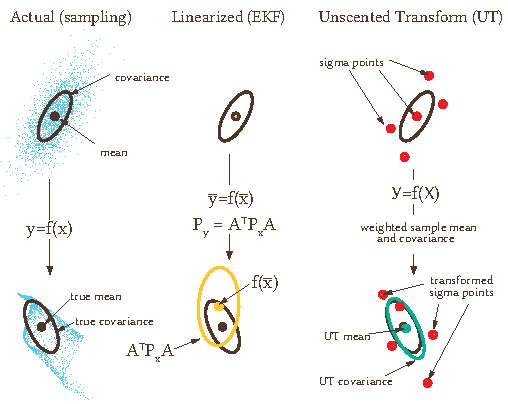
\includegraphics[width=\linewidth]{unscented_transform}
\end{minipage}
\end{figure}

\subsection{Quadrature-type Kalman Filters (QKF, CKF)} \index{Quadrature Kalman Filter}
The integrals \eqref{e:s1:adf:mux}, \eqref{e:s1:adf:pxx}, and \eqref{e:s1:adf:mux} can also be approximated with the Gauss--Hermite quadrature rule~\cite{Nay82}:  \index{integration techniques!quadrature}
\begin{equation} \label{e:s1:GHquad}
\int \eta(z;0,1) f(z) \approx \sum_{i=1}^m w_i f(\mu+\sqrt{2}\sigma z_i).
\end{equation}
Such an approximation is exact when $f$ is a polynomial of degree less than $m$, where the weights $w_i$ and knots $z_i$ are given in~\cite{Gol73}.  A simple change of variables can be used to generalize \eqref{e:s1:GHquad} to nonstandard normal distributions.  \textcite{Ito00b} extend this rule to multivariate quadrature:
\begin{equation} \label{e:s1:GHmultiv}
\int \eta_d(z;0,S) f(z) \approx \sum_{i_1=1}^m \dotsb \sum_{i_d=1}^m w_{i_1}\dotsb w_{i_d} f(q_{i_1},\dotsc, q_{i_d})
\end{equation}
for specified weights $w_{i_j}$ and knots $q_{i_j}$. Such a rule is exact for all polynomials of multidegree up to $(2m-1,\dotsc,2m-1)$.  Using the above quadrature rule for integration in this filtering model yields the Quadrature Kalman filter of~\textcite{Cha00,Ito00b}.  The spherical-radial cubature rule implements a cubature scheme to the same effect~\cite[the Cubature--Quadrature Kalman filter of][]{Ara07,Ara09}.

%%%%%%%%%%%%%%%%%%%%%%%%%%%%%%%%%%%%%%%%%%%%%%%%%
\begin{figure}[h]
\begin{minipage}[c]{.32\textwidth}
\includegraphics[width=\linewidth]{q1}
\end{minipage}
\hfill
\begin{minipage}[c]{.32\textwidth}
\includegraphics[width=\linewidth]{q2}
\end{minipage}
\hfill
\begin{minipage}[c]{.32\textwidth}
\includegraphics[width=\linewidth]{q3}
\end{minipage}
\caption[The Midpoint Quadrature Rule]{The Midpoint Quadrature Rule approximates an integral by partitioning the domain of integration and approximating the integral over each partition $[a,b]$ as $\int_a^b f(x)\; dx \approx (b-a)\cdot f(\tfrac{a+b}{2})$.  Such an approximation improves as the partition becomes finer.}
\end{figure}

\subsection{Fourier--Hermite Kalman Filter (FHKF)} \index{Fourier--Hermite Kalman Filter}
The integrals \eqref{e:s1:adf:mux}, \eqref{e:s1:adf:pxx}, and \eqref{e:s1:adf:mux} can also be approximated as a Fourier--Hermite expansion~\cite{Sar12}.

\subsection{Related Work}
It is possible to propagate the first two moments for the Gaussian posterior using particle filtering~\cite{Kot03b} or even a Gaussian process~\cite{Ko07,Ko09}.

%%%%%%%%%%%%%%%%%%%%%%%%%%%%%%%%%%%%%%%%%%%%%%%%%
\section{The Particle Filter (PF)} \label{s:PF} \index{particle filter} \index{integration techniques!Monte Carlo}
\textcite{Met49} developed the Monte Carlo method for numerical integration.  The idea is to replace integration with summation, i.e. for $f\in L^1(dp)$:
\begin{equation}
\Exp[f(Z)] = \int f(z)\; p(z)\; dz \approx \frac{1}{N} \sum_{i=1}^N f(Z_i)
\end{equation}
where $Z,Z_1,\dotsc, Z_N\sim^\text{i.i.d.} p$.  The Strong Law of Large Numbers implies that the approximation error tends to zero a.s. as $N\to\infty$.  If it is easier to draw samples from some p.d.f. $q$ where $q\ll p$ ($q$ is absolutely continuous with respect to $p$), then we obtain importance sampling:
\begin{equation} \label{e:s1:IS}
\Exp[f(Z)] = \int f(z)\; \frac{p(z)}{q(z)}\; q(z)\; dz \approx \frac{1}{N} \sum_{i=1}^N f(Z_i)\frac{p(Z_i)}{q(Z_i)}.
\end{equation}
By optimizing over possible sampling distributions, it is also possible to use this method to reduce variance for the approximation.  Applying the importance sampling approximation in \eqref{e:s1:IS} to the Chapman--Kolmogorov recursion in \eqref{e:s1:BFalt} yields Sequential importance sampling (SIS)~\cite{Han69,Han70,Kit96,del96,Dou00,Cap05,Cap07}.  \index{particle filter!Sequential Importance Sampling} 

%%%%%%%%%%%%%%%%%%%%%%%%%%%%%%%%%%%%%%%%%%%%%%%%%
\begin{figure}[h]
\begin{minipage}[c]{.49\textwidth}
\includegraphics[width=\linewidth]{sis}
\end{minipage}
\hfill
\begin{minipage}[c]{.49\textwidth}
\caption[Sequential Importance Sampling]{A. We start with a particle representation of $p(z_{t-1}|x_{1:t-1})$.  B. The location of each particle is updated according to $p(z_t|z_{t-1})$.  C. The weight of each particle is updated according to $p(x_t|z_t)$.  Weights are renormalized to sum to $1$.  We now have a particle representation of $p(z_t|x_{1:t})$.}
\end{minipage}
\end{figure}

We outline the Sequential Importance Resampling (SIR) method pioneered by~\cite{Gor93}.  \index{particle filter!Sequential Importance Resampling} We first represent $p(z_{t-1}|x_{1:t-1})$ as a sum of weighted particles
\begin{equation}
p(z_{t-1}|x_{1:t-1}) \approx \sum_{\ell=1}^L w_{t-1}^{(\ell)} \delta_{z_{t-1}^{(\ell)}}(z_{t-1}). \label{e:s1:PF}
\end{equation}
At each step in the recursion, we resample $z_{t-1}^{(\ell)}$ according to the weights $w_{t-1}^{(\ell)}$ to obtain equally-weighted samples $\tilde z_{t-1}^{(\ell)}$.  This resampling prevents particle collapse (an issue where the vast majority of particles are assigned negligible weight so that the number of effective particles becomes very small)  and gives us a modified form of \eqref{e:s1:BF}:
\begin{equation}
p(z_t|x_{1:t}) \propto   \sum_{\ell=1}^L p(x_t|z_t^{(\ell)}) \int p(z_t|y)   \delta_{\tilde z_{t-1}^{(\ell)}}(y) \; dy.
\end{equation}
(The resampling step is what distinguishes SIR from SIS. ) We then sample $z_t^{(\ell)}$ from
\begin{equation} \label{e:s1:PF_loci}
Z_{t}^{(\ell)} \sim Z_t|\{Z_{t-1}=\tilde z_{t-1}^{(\ell)}\}
\end{equation}
so that
\begin{equation*}
p(z_t|x_{1:t-1}) \approx \sum_{\ell=1}^L  \delta_{z_t^{(\ell)}}(z_t)
\end{equation*}
and then update the weights
\begin{equation} \label{e:s1:PF_weights}
w_t^{(\ell)} \propto p(x_t|z_{t}^{(\ell)}).
\end{equation}
Weights are normalized to sum to 1 and this yields our next representation in the form of \eqref{e:s1:PF}.

%%%%%%%%%%%%%%%%%%%%%%%%%%%%%%%%%%%%%%%%%%%%%%%%%
\begin{figure}[h]
\begin{minipage}[c]{.49\textwidth}
\caption[Sequential Importance Resampling]{A. We start with a particle representation of $p(z_{t-1}|x_{1:t-1})$.  B. Particles are selected with replacement according to their relative weights.  This gives us a new set of particles that are now equally weighted.  C. The location of each particle is updated according to $p(z_t|z_{t-1})$.  D. The weight of each particle is updated according to $p(x_t|z_t)$.  Weights are renormalized to sum to $1$, yielding a particle representation of $p(z_t|x_{1:t})$.}
\end{minipage}
\hfill
\begin{minipage}[c]{.49\textwidth}
\includegraphics[width=\linewidth]{sir}
\end{minipage}
\end{figure}

\subsection{Related Work}
Alternate sampling strategies~\cite[see, e.g.,][]{Che03,Liu08} can be used to improve filter performance, including: acceptance-rejection sampling~\cite{Han69}, stratified sampling~\cite{Dou05}, hybrid MC~\cite{Cho01}, and quasi-MC~\cite{Ger15}.

There are also ensemble versions of the Kalman filter that are used to propagate the covariance matrix in high state-dimensions including the ensemble Kalman filter~\cite[enKF:][]{Gei94} and ensemble transform Kalman filter~\cite[ETKF:][]{Bis01,Maj02}, along with versions that produce local approximations for covariance and can be parallelized~\cite{Ott02,Ott04,Hun07}.  These filters seem well-suited to climate modeling. 

Recent innovations include: the auxiliary particle filter that introduces an auxiliary variable to increase sampling efficiency and robustness to outliers~\cite{Pit99}, introducing block sampling techniques to particle filters~\cite{Dou06}, resample--move algorithms that increase particle diversity without changing the estimated distribution~\cite{Gil01}, and MCMC moves within particle filters~\cite{And10}.

Many of the algorithms mentioned in previous sections can be reformulated with a particle filter-based integral approximation: the unscented particle filter~\cite{van01b},
the sigma-point particle filter~\cite{van04}, the Gaussian mixture sigma-point particle filter~\cite{van03}, and a Laplace method-inspired particle filter~\cite{Qua16}.

%%%%%%%%%%%%%%%%%%%%%%%%%%%%%%%%%%%%%%%%%%%%%%%%%
\begin{figure}[h]
\begin{minipage}[t]{.45\textwidth}
\includegraphics[width=\linewidth]{ecmwf-ensemble_earths}
\caption[An Ensemble of Earths]{Particles in a particle filter can represent a wide range of things, from global atmospheric conditions to phylogenetic trees~\cite{Bou12,Wan15,Din18}. Image credit: European Centre for Medium-Range Weather Forecasts.}
\end{minipage}%
\hfill
\begin{minipage}[t]{.45\textwidth}
\includegraphics[width=\linewidth]{ecmwf-ensemble}
\caption[An Ensemble Weather Forecast, Illustrated]{Weather forecasts assimilate data with ensemble versions of the Kalman filter~\cite{Gei94,Bis01,Ott04,Hun07,Bue17}.  Image credit: European Centre for Medium-Range Weather Forecasts.}
\end{minipage}
\end{figure}

%%%%%%%%%%%%%%%%%%%%%%%%%%%%%%%%%%%%%%%%%%%%%%%%%
\section{Filtering Innovations} 

We describe here some meta-methods used to improve filter performance than have proven successful across multiple filter types.

\subsection{Square-Root Transform} \index{square-root filters}
Various decompositions of the covariance estimate have been used to ensure positive-definiteness and obtain better matrix conditioning in filter recursions.  The idea is to store and update the matrix square root of the covariance estimate instead of the covariance estimate itself, thereby working with a matrix that automatically yields a positive-definite covariance estimate and that possesses a condition number that is the square root of the original~\cite{And79}. \textcite{Pot63} pioneered the approach with the Cholesky decomposition and scalar-valued observations; \textcite{Bel67} extended the algorithm to multidimensional observations.

Note that \eqref{e:s1:phit_reln} is equivalent to:
\begin{equation}
(\Phi_t)^{-1} = (\hat\Phi_{t-1})^{-1} + H^\intercal\Lambda^{-1}H.
\end{equation}
With the following Cholesky decompositions
\begin{align}
\hat\Phi_{t-1} &= PP^\intercal \\
\Lambda &= LL^\intercal
\end{align}
it becomes
\begin{align}
(\Phi_t)^{-1} 
&= (PP^\intercal)^{-1} + H^\intercal(L^{-1})^\intercal L^{-1}H \\
&= (P^{-1})^\intercal (I_d+BB^\intercal) P^{-1}
\end{align}
where $B = (L^{-1}HP)^\intercal$.  Taking inverses then yields:
\begin{equation}
\Phi_t = P(I_d+BB^\intercal)^{-1}P^\intercal
\end{equation}
and the Kalman gain is given by
\begin{equation}
K_t = PB(I_d+B^\intercal B)^{-1}L^{-1}
\end{equation}
Subsequent work generalized it further~\cite{And68,Sch70b,Kam71}, including the use of other decompositions such as QR~\cite{Say93,Say94}, Householder~\cite{Dye69,Car73}, and U-D~\cite{Bie75,Tho76}.  Square-root versions have also been developed for the UKF and CDKF~\cite{van01}.

\subsection{Rao--Blackwellization} \index{Rao--Blackwell theorem} 
The Rao--Blackwell theorem states that, given an unbiased estimator $\hat\theta$ and a sufficient statistic $T$ for some random variable $\theta$, the estimator $\tilde\theta:= \Exp[\hat\theta|T]$ is unbiased and~\cite{Cas01}
\[
\var_\theta[\tilde\theta]\leq \var_\theta[\hat\theta],
\]
i.e. conditioning an estimator with a sufficient statistic reduces variance.  This notion can be applied to Bayesian particle filtering by finding a decomposition of the latent state  model into a part that can be integrated exactly (with a Kalman filter) and a remaining (now smaller) part to which particle filtering is applied.  This is the idea underlying Rao--Blackwellized particle filtering~\cite{Dou00,Dou00b}.

\subsection{Gaussian Sum and Mixture Models} 
To extend the class of models under consideration, it is common to reformulate a Gaussian filter to handle a mixture of Gaussians.  The filter then propagates each Gaussian component separately, allowing for a richer representation of the posterior distribution~\cite{Sor71,Als72,Tam99, Che00,Ter11}.  This approach has even be combined with other methods, such as the Gaussian sum particle filter~\cite{Kot03} and the Gaussian-sum Quadrature Kalman Filter~\cite{Ara07}.

\subsection{Dual Filtering}
It is sometimes desirable to infer states and update model parameters simultaneously.  Dual (Extended) Kalman filtering refers to a method to accomplish this~\cite{Nel97,Wan97,Wan00b}.

%\subsection{Applications}
% The Apollo program~\cite{Hal66, Bat70, Gre10}, C-5 guidance~\cite{Sch70}, neural filtering [will be covered elsewhere].
